\chapter{Infrastruktur}
\label{infrastruktur}

\todo[inline]{Server-Setup dokumentieren (Virtueller Server, Travis, heroku etc.}
\section{Architektur}

Das Gesamtsystem setzt sich aus insgesamt vier Komponenten zusammen: die Datenbank, der Webserver, die Fehlerquelle und das Zielsystem von OpenStreetMap. 
Die einzelnen Komponenten sind über \gls{REST}-Schnittstellen miteinander verbunden. 
Dabei sind das Zielsystem (OpenStreetMap) und die Fehlerquelle (Keepright, siehe Kapitel \ref{datenquellen}) Fremdsysteme, bei welchen die Schnittstellen gegeben waren. 
Unsere eigenen Server haben wir entsprechend angepasst und auch via REST zugänglich gemacht.

\begin{figure}[H]
\subfigure[Gesamtübersicht der Systeme]{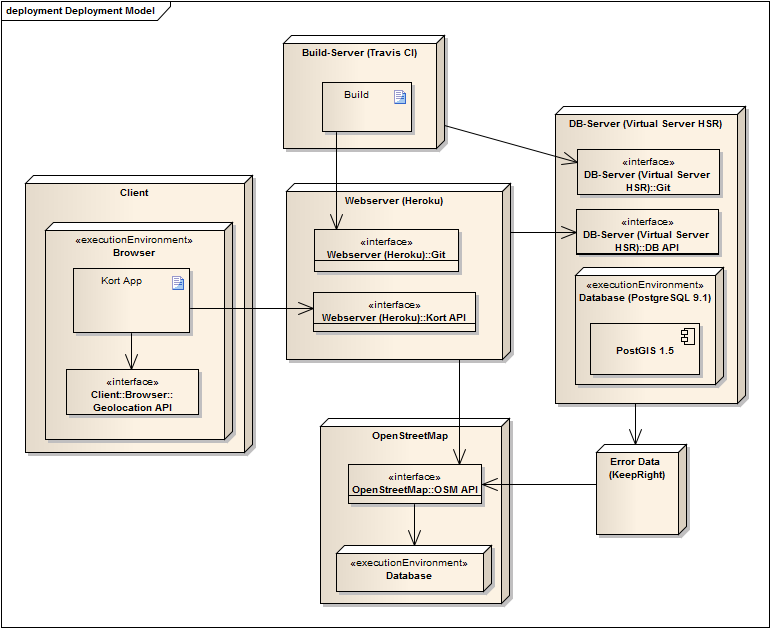
\includegraphics[width=\textwidth]{images/uml/deployment_diagram.png}}
\end{figure}

\subsection{REST-Schnittellen}
Die Entscheidung \gls{REST}-Schnittstellen zu verwenden haben wir schnell gefasst. 
Zum einen ist damit eine einheitliche Schnittstelle im gesamten System vorhanden, so dass immer klar ist über welchen Kanal eine Kommunikation passiert.
Zum anderen sind \gls{REST}-Schnittellen für Webapplikation sehr einfach zu verwenden, da entsprechende Bibliotheksfunktionen bereits vorhanden sind.
Schlussendlich ist entscheidend, dass \gls{REST}-Schnittstellen ein grosses Mass an Plattformunabhängigkeit bieten und so die räumliche Teilung der Systeme erleichtert.

\section{Datenbankserver}

Beim Datenbankserver handelt es sich um einen virtuellen Server, den uns die Hochschule für Technik Rapperswil (HSR) zur Verfügung gestellt hat für die Dauer dieser Arbeit.

\begin{table}[H]
\centering
\begin{tabular}{|p{0.25\twocelltabwidth}|p{0.75\twocelltabwidth}|}
\hline 
\textbf{Art des Servers} & Virtueller Server \\
\hline 
\textbf{Betriebsystem} & Ubuntu 12.04 (LTS) \\
\hline 
\textbf{Zugriff} & Root-Zugriff via SSH \\
\hline 
\textbf{Installierte Software} & PostgreSQL 9.1, PostGIS 2.0, Redmine 2.1 \\
\hline 
\end{tabular} 
\caption{Datenbankserver der Hochschule für Technik Rapperswil}
\label{infrastruktur-datenbankserver-tabelle}
\end{table}

\section{Webserver (Heroku)}

Bei Heroku\footnote{\url{http://www.heroku.com/}} handelt es sich um einen kostenlosen Dienst, welcher für verschiedenste Plattformen eine Deploymentumgebung anbietet. 
Der Dienst hat eine Schnittstelle über welche sich automatisiert Applikationen erstellen lassen, die Datenübertragung läuft dann über \gls{git}.

\begin{table}[H]
\centering
\begin{tabular}{|p{0.25\twocelltabwidth}|p{0.75\twocelltabwidth}|}
\hline 
\textbf{Art des Servers} & Server in der \gls{Cloud} \\
\hline 
\textbf{Betriebsystem} & Ubuntu \\
\hline 
\textbf{Zugriff} & Daten via \gls{git}, Befehle via Kommandozeilen-API (Heroku Toolbelt) \\
\hline 
\textbf{Installierte Software} & Apache, kort Applikation \\
\hline 
\end{tabular} 
\caption{Server bei Heroku}
\label{infrastruktur-heroku-tabelle}
\end{table}

\section{Deployment}
Am Deployment der Applikation sind mehrere Systeme beteiligt. 
Alle Änderungen werden von den Entwicklern via \gls{git} zu GitHub\footnote{\url{http://github.com}} übertragen. 
Auf GitHub gibt es sogenannte Hooks die man aktivieren kann. 
Dabei handelt es sich um weitere Aktionen welche durch verschiedene Ereignisse ausgelöst werden können. 
In unserem Fall haben wir einen \emph{post-commit Hook} aktiviert, welcher dem \gls{ci} Dienst Travis-CI\footnote{\url{http://travis-ci.org}} Bescheid gibt, wenn ein neue Änderungen auf GitHub eingetroffen sind.

Auf Travis läuft dann der Build, welcher durch die Konfigurationsdatei \inlinecode{.travis.yml} gesteuert ist. Darin lassen wir die Schritte sowie die Umgebung für Builds definieren. Für jede Umgebung wird dann ein separater Build ausgelöst. Somit lassen sich bequem verschiedene Versionen mit unterschiedlichen Umgebungen testen (siehe Tabelle \ref{infrastruktur-build-matrix}).

\begin{table}[H]
\centering
\begin{tabular}{|p{0.2\threecelltabwidth}|p{0.4\threecelltabwidth}|p{0.4\threecelltabwidth}|}
\hline 
 & \textbf{Test} & \textbf{Produktion} \\
\hline 
\textbf{PHP 5.3} & Build und Test & Build und Test \\
\hline 
\textbf{PHP 5.4} & Build, Test und Deployment auf \url{http://kort-dev.herokuapp.com} & Build, Test und Deployment auf \url{http://kort.herokuapp.com} \\
\hline 
\end{tabular} 
\caption{Build-Matrix von Travis CI}
\label{infrastruktur-build-matrix}
\end{table}
